\documentclass[12pt,twoside]{report}

%%%%%%%%%%%%%%%%%%%%%%%%%%%%%%%%%%%%%%%%%%%%%%%%%%%%%%%%%%%%%%%%%%%%%%%%%%%%%

% Definitions for the title page
% Edit these to provide the correct information
% e.g. \newcommand{\reportauthor}{Timothy Kimber}

\newcommand{\reporttitle}{Title}
\newcommand{\reportauthor}{Your name}
\newcommand{\supervisor}{Name of supervisor}
\newcommand{\degreetype}{Type of Degree}

%%%%%%%%%%%%%%%%%%%%%%%%%%%%%%%%%%%%%%%%%%%%%%%%%%%%%%%%%%%%%%%%%%%%%%%%%%%%%

% load some definitions and default packages
%%%%%%%%%%%%%%%%%%%%%%%%%%%%%%%%%%%%%%%%%
% University Assignment Title Page 
% LaTeX Template
% Version 1.0 (27/12/12)
%
% This template has been downloaded from:
% http://www.LaTeXTemplates.com
%
% Original author:
% WikiBooks (http://en.wikibooks.org/wiki/LaTeX/Title_Creation)
%
% License:
% CC BY-NC-SA 3.0 (http://creativecommons.org/licenses/by-nc-sa/3.0/)
% 
%
%%%%%%%%%%%%%%%%%%%%%%%%%%%%%%%%%%%%%%%%%
%----------------------------------------------------------------------------------------
%	PACKAGES AND OTHER DOCUMENT CONFIGURATIONS
%----------------------------------------------------------------------------------------
\usepackage[a4paper,hmargin=2.8cm,vmargin=2.0cm,includeheadfoot]{geometry}
\usepackage{textpos}
\usepackage[nottoc]{tocbibind} % for bibliography
\usepackage{tabularx,longtable,multirow,subfigure,caption}%hangcaption
\usepackage{fncylab} %formatting of labels
\usepackage{fancyhdr} % page layout
\usepackage{url} % URLs
\usepackage[english]{babel}
\usepackage{amsmath}
\usepackage{graphicx}
\usepackage{dsfont}
\usepackage{epstopdf} % automatically replace .eps with .pdf in graphics
\usepackage{backref} % needed for citations
\usepackage{array}
\usepackage{latexsym}
\usepackage[pdftex,pagebackref,hypertexnames=false,colorlinks]{hyperref} % provide links in pdf
\usepackage{parskip}
\usepackage{float}
\usepackage{makecell}
\usepackage{xcolor}

% code type
\definecolor{light-gray}{gray}{0.95}
\newcommand{\code}[1]{\colorbox{light-gray}{\texttt{#1}}}

\hypersetup{pdftitle={},
  pdfsubject={}, 
  pdfauthor={},
  pdfkeywords={}, 
  pdfstartview=FitH,
  pdfpagemode={UseOutlines},% None, FullScreen, UseOutlines
  bookmarksnumbered=true, bookmarksopen=true, colorlinks,
    citecolor=black,%
    filecolor=black,%
    linkcolor=black,%
    urlcolor=black}

\usepackage[all]{hypcap}


%\usepackage{color}
%\usepackage[tight,ugly]{units}
%\usepackage{float}
%\usepackage{tcolorbox}
%\usepackage[colorinlistoftodos]{todonotes}
% \usepackage{ntheorem}
% \theoremstyle{break}
% \newtheorem{lemma}{Lemma}
% \newtheorem{theorem}{Theorem}
% \newtheorem{remark}{Remark}
% \newtheorem{definition}{Definition}
% \newtheorem{proof}{Proof}


%%% Default fonts
\renewcommand*{\rmdefault}{bch}
\renewcommand*{\ttdefault}{cmtt}



%%% Default settings (page layout)
\setlength{\parindent}{0em}  % indentation of paragraph

\setlength{\headheight}{14.5pt}
\pagestyle{fancy}
\renewcommand{\chaptermark}[1]{\markboth{\chaptername\ \thechapter.\ #1}{}} 

\fancyfoot[ER,OL]{\sffamily\textbf{\thepage}}%Page no. in the left on odd pages and on right on even pages
\fancyfoot[OC,EC]{\sffamily }
\renewcommand{\headrulewidth}{0.1pt}
\renewcommand{\footrulewidth}{0.1pt}
\captionsetup{margin=10pt,font=small,labelfont=bf}


%--- chapter heading

\def\@makechapterhead#1{%
  \vspace*{10\p@}%
  {\parindent \z@ \raggedright \sffamily
    \interlinepenalty\@M
    \Huge\bfseries \thechapter \space\space #1\par\nobreak
    \vskip 30\p@
  }}

%---chapter heading for \chapter*  
\def\@makeschapterhead#1{%
  \vspace*{10\p@}%
  {\parindent \z@ \raggedright
    \sffamily
    \interlinepenalty\@M
    \Huge \bfseries  #1\par\nobreak
    \vskip 30\p@
  }}

\allowdisplaybreaks

% load some macros
% Here, you can define your own macros. Some examples are given below.

\newcommand{\R}[0]{\mathds{R}} % real numbers
\newcommand{\Z}[0]{\mathds{Z}} % integers
\newcommand{\N}[0]{\mathds{N}} % natural numbers
\newcommand{\C}[0]{\mathds{C}} % complex numbers
\renewcommand{\vec}[1]{{\boldsymbol{{#1}}}} % vector
\newcommand{\mat}[1]{{\boldsymbol{{#1}}}} % matrix


\date{\today}

\begin{document}

% load title page
% Last modification: 2015-08-17 (Marc Deisenroth)
\begin{titlepage}

\newcommand{\HRule}{\rule{\linewidth}{0.5mm}} % Defines a new command for the horizontal lines, change thickness here


%----------------------------------------------------------------------------------------
%	LOGO SECTION
%----------------------------------------------------------------------------------------


\includegraphics[width = 4cm]{./figures/imperial}\\[0.5cm] 

\center % Center remainder of the page

%----------------------------------------------------------------------------------------
%	HEADING SECTIONS
%----------------------------------------------------------------------------------------

\textsc{\Large Imperial College London}\\[0.5cm] 
\textsc{\large Department of Computing}\\[0.5cm] 

%----------------------------------------------------------------------------------------
%	TITLE SECTION
%----------------------------------------------------------------------------------------

\HRule \\[0.4cm]
{ \huge \bfseries \reporttitle}\\ % Title of your document
\HRule \\[1.5cm]
 
%----------------------------------------------------------------------------------------
%	AUTHOR SECTION
%----------------------------------------------------------------------------------------

\begin{minipage}{0.4\textwidth}
\begin{flushleft} \large
\emph{Author:}\\
\reportauthor % Your name
\end{flushleft}
\end{minipage}
~
\begin{minipage}{0.4\textwidth}
\begin{flushright} \large
\emph{Supervisor:} \\
\supervisor % Supervisor's Name
\end{flushright}
\end{minipage}\\[4cm]


%----------------------------------------------------------------------------------------
%	FOOTER & DATE SECTION
%----------------------------------------------------------------------------------------
\vfill % Fill the rest of the page with whitespace
Submitted in partial fulfillment of the requirements for the MSc degree in
\degreetype~of Imperial College London\\[0.5cm]

\makeatletter
\@date 
\makeatother


\end{titlepage}



% page numbering etc.
\pagenumbering{roman}
\clearpage{\pagestyle{empty}\cleardoublepage}
\setcounter{page}{1}
\pagestyle{fancy}

%%%%%%%%%%%%%%%%%%%%%%%%%%%%%%%%%%%%
\begin{abstract}
Your abstract.
\end{abstract}

\cleardoublepage
%%%%%%%%%%%%%%%%%%%%%%%%%%%%%%%%%%%%
\section*{Acknowledgments}
Comment this out if not needed.

\clearpage{\pagestyle{empty}\cleardoublepage}

%%%%%%%%%%%%%%%%%%%%%%%%%%%%%%%%%%%%
%--- table of contents
\fancyhead[RE,LO]{\sffamily {Table of Contents}}
\tableofcontents 


\clearpage{\pagestyle{empty}\cleardoublepage}
\pagenumbering{arabic}
\setcounter{page}{1}
\fancyhead[LE,RO]{\slshape \rightmark}
\fancyhead[LO,RE]{\slshape \leftmark}

%%%%%%%%%%%%%%%%%%%%%%%%%%%%%%%%%%%%
\chapter{Introduction}
\label{Introduction}

%\begin{figure}[tb]
%\centering
%
\includegraphics[width = 0.4\hsize]{./figures/imperial}
%%\caption{Imperial College Logo. It's nice blue, and the font is quite stylish. But you can choose a different one if you don't like it.}
%\label{fig:logo}
%\end{figure}

%Figure~\ref{fig:logo} is an example of a figure. 
\begin{figure}
    \centering
    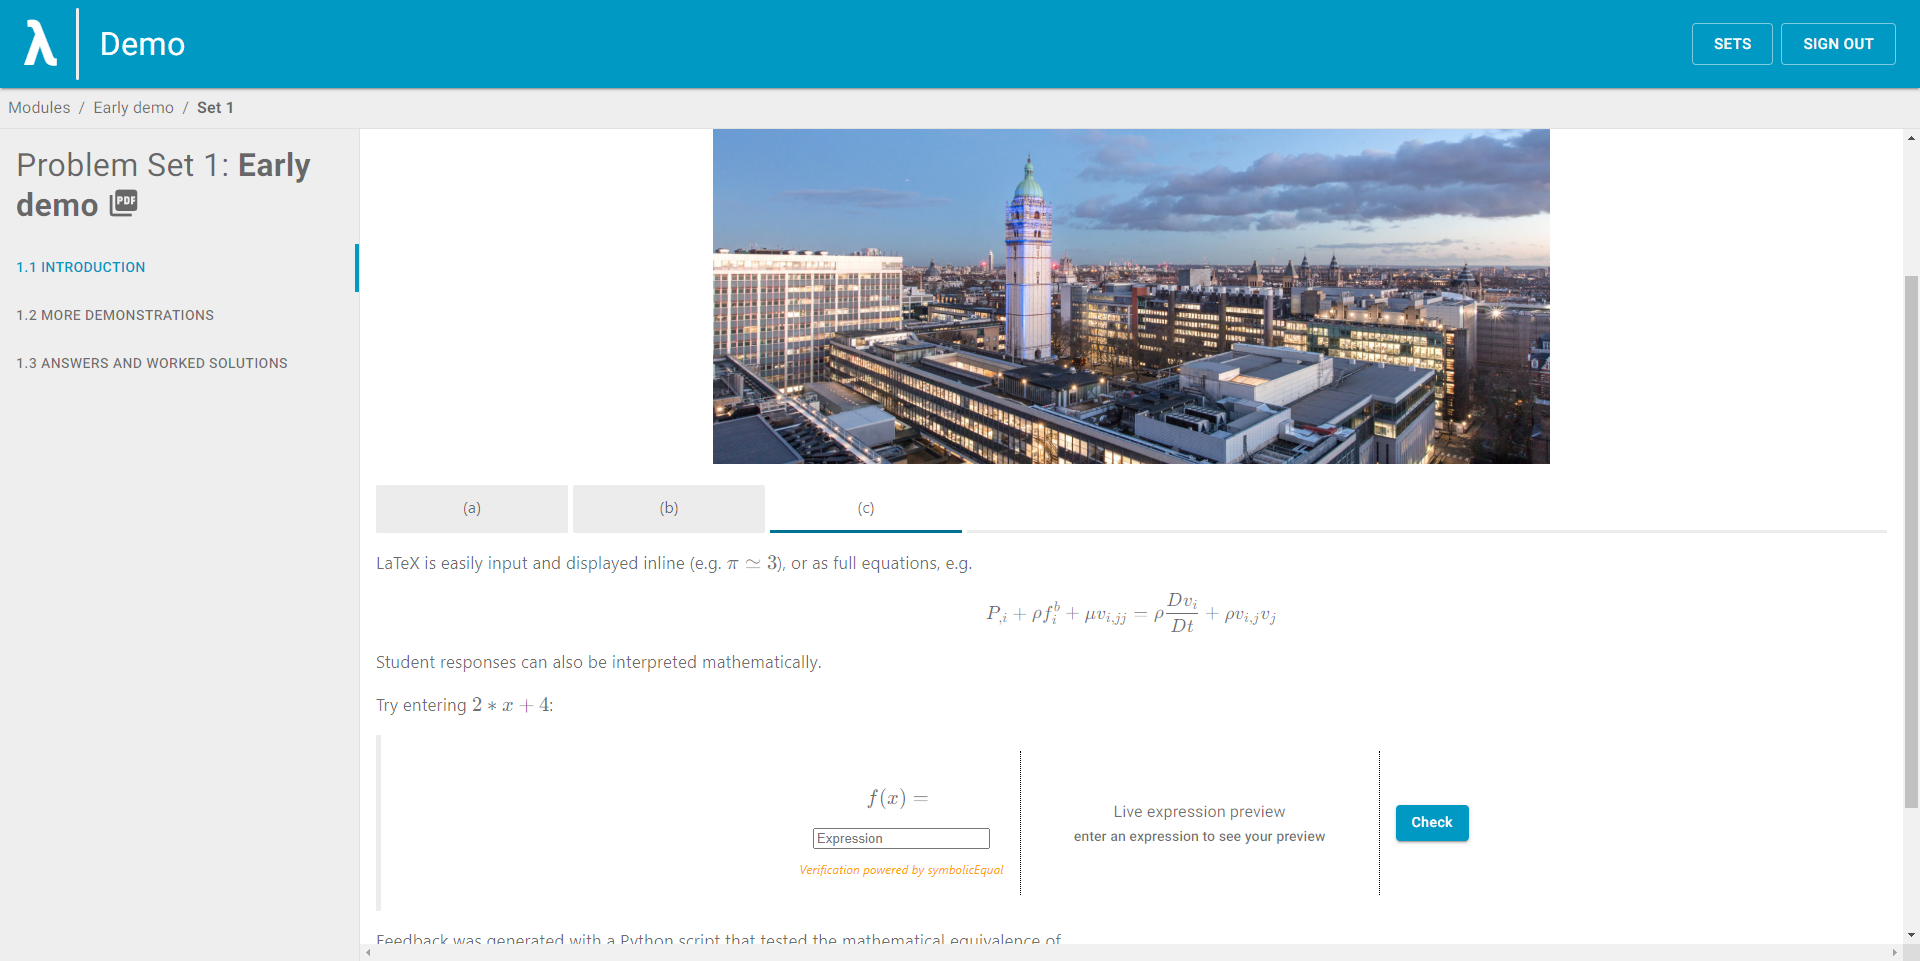
\includegraphics[width=\hsize]{figures/lambdafeedback-screenshot.png}
    \caption{Screenshot of a Demo in Lambada Feedback System}
    \label{fig:demoscreenshot}
\end{figure}

The application of remote learning in higher education has increased massively
since the explosion of COVID-19 \cite{remotelearning}. Many institutions including Imperial College
London moved their courses online during lockdowns. These courses are taught
based on online systems. However, some online systems are not capable of
conducting the digitalisation of teaching tasks such as lecture
recording/playing and assignment marking etc. For example, some departments of  Imperial College
London were using Möbius for online assignment and assessment, but it was complained by students and staffs that the system was hard to use. This thus leads to a demand of updating or developing new systems so that students and teachers can get better experience.

Therefore, the college has decided to develop a new online learning system named
Lambda Feedback. This system is a web application which allows students to do assignments posted by teachers and get feedback immediately. Comparing to its predecessor Möbius, Lambda
Feedback has modern user interface, friendly interaction and much more features.
One of the features is the expression input. In many assignment questions,
solutions are math expressions. In Lambda Feedback, users can input math
expressions in a text field, and the system is able to understand the expression
and check if it is correct. Figure \ref{fig:demoscreenshot} is a screenshot of a
demo in Lambda Feedback. The webpage displays a navigation sidebar,
the question, and the answer area, where users can input the expression.

However, the current system only supports keyboard input for math expressions.
Users need to type the whole expression including symbols and operators, which
can be very inconvenient and complex especially for complicated equations.
Consequently, an extension with a new method of input is needed for the system.

Handwriting input is considered appropriate for the system because of its
convenience and simplicity. Although there are other input methods such as
equation editor and image upload, they either require users to learn how to use,
or need some extra steps. This means they are not suitable as the major approach
of expression input, but can be a good supplement to handwriting input in some
special situations.

This project thus aims to develop a component with handwriting input and
equation recognition, and integrate it to the Lambda Feedback system. The
component shall enable the users to write on it either via mouse/touchpad on
computers or fingers/pens on mobile devices. After users finish a stroke, it should
be able to recognize the equation and display the result alongside the writing
area. Integration with the Lambda Feedback system should be carried out after
the component is tested available.

This report records the development of the project. Chapter \ref{Background}
investigates several approaches to realise the software component and analyses
their advantages and drawbacks. Chapter \ref{Implementation} states the process
of development and explains the implementation of the software component. In
Chapter \ref{Results}, progressive results are demonstrated and the final
achievement is shown. An evaluation of the results are included in this chapter
as well. Finally, in chapter \ref{Conclusion}, a conclusion of the project is drawn, and possible future improvements are listed.



%%%%%%%%%%%%%%%%%%%%%%%%%%%%%%%%%%%%
\chapter{Background}
\label{Background}

This chapter records the background research, which includes general reviews on
articles, tutorials and existing projects that have helped the development of
this project, as well as potential choices that could be taken and why they were
discarded, along with the reasons of selecting current tools. An overview of the project is made below before diving into details.

\section*{Overview}
\label{bgOverview}

The component to develop is a TypeScript (strong typed version of JavaScript) web application which has two major functionalities:
\begin{enumerate}
    \item Have a canvas where users can write equation
    \item Ability to recognise the equation written on canvas and display the result
\end{enumerate}

In addition, the application should include some functions for editing the user's drawing, such as undo, redo, delete all and remove stroke.

Moreover, the component should be integrated into Lambda Feedback, so it is necessary to introduce the system because they will use same frameworks and language.

Lambda Feedback is a web application which has a frontend and a backend.
The frontend is built upon NextJS (a framework built on React), and the backend is built upon NestJS. Both
are written in Typescript (These frameworks will be introduced in Chapter \ref{bgIntegrationLF}). Most code of the project will be installed in a component of the frontend named \code{ResponseArea}, which is responsible for receiving input and giving result to users.

It is difficult to develop the component directly upon Lambda Feedback, as it
already had much code when this project launched. Therefore, it was decided to
build a web application independent of Lambda Feedback to save time on reading
code and testing functionality.

Although the final independent web application must be written under the same
framework with Lambda Feedback, i.e. React, there is another way,
Vanilla JavaScript (also referred to as plain JS), to start with. Table \ref{MethodComparison} compares the two methods:
\begin{table}[H]
    \centering
    \caption{Comparison of Two Methods for Independent Web Application}
    \label{MethodComparison}
    \begin{tabular}{|m{0.15\textwidth}|m{0.4\textwidth}|m{0.3\textwidth}|}
        \hline
        \textbf{Method} & \textbf{Advantages} & \textbf{Disadvantages}\\
        \hline
        Vanilla JS & Easy to start \& Require no extra configuration&
        Does not fit Lambda Feedback\\
        \hline
        React & Uses same framework as Lambda Feedback - does not need extra steps for integration & Need to study React before start\\
        \hline
    \end{tabular}
\end{table}
After careful consideration, it was decided to start by using Vanilla JS to get familiar with functionalities, and then converting the application to React. This makes the procedure more fluent and only need to focus on one emphasis for every update.

Overall, the procedure of the project is:
\begin{enumerate}
    \item Develop a web application with Vanilla JS which enables users to draw equations, and recognise the equation
    \item Move the web application under React framework
    \item Integrate the application as a component to Lambda Feedback
\end{enumerate}


Despite using different frameworks during the procedure, the approaches to realise functionalities are the same. Hence, the background research mainly focuses on three parts:
\begin{itemize}
    \item React framework and integration with the Lambda Feedback
    \item A canvas where users can draw stuffs
    \item Functionality of mathematical equation recognition
\end{itemize}
Therefore, the remaining part of this chapter is divided into three sections, each introducing one part. 

\section{React and Lambda Feedback}
\label{bgIntegrationLF}
Lambda Feedback's frontend is built upon NextJS, a framework based on
React. Distinct features of NextJS mainly focus on page level
optimization, and the method of building a component remains the same as
React. Therefore, it is necessary to learn React framework
before building the component for Lambda Feedback, but only need to have a
general understanding of NextJS.

React is an open-source frontend library deployed to develop reusable user interface (UI) components. Unlike Vanilla JS which structures all the layouts of a webpage in one file, React focuses on the idea of components \cite{rawat2020reactjs}. 

In Vanilla JS, layouts, functions and styles of a webpage are written in HTML, JS and CSS file respectively. However, in React, the webpage is assembled by React components. This makes component the basic unit in React. Layout and functions of a component are in the same file whose type is JSX. Even styles can be embedded in it as well. This means only one file is needed for one component \cite{rawat2020reactjs}. Figure \ref{fig:vanillajs-react-compare} shows the design pattern of VanillaJS and React. 
\begin{figure}[h]
    \centering
    \begin{subfigure}{0.7\linewidth}
        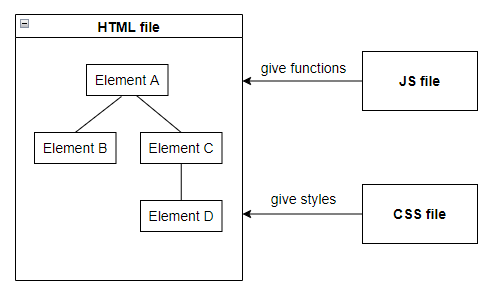
\includegraphics[width=\linewidth, frame]{figures/vanillajs-design-pattern.png}
        \caption{Design Pattern of Vanilla JS}
        \label{fig:vanillajs-design-pattern}
    \end{subfigure}
    \begin{subfigure}{0.7\linewidth}
        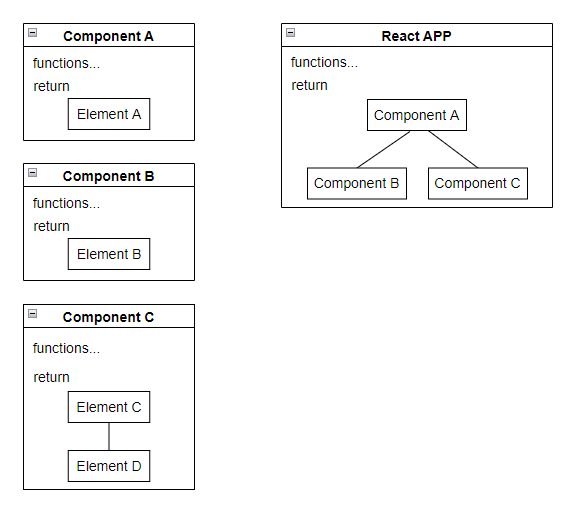
\includegraphics[width=\linewidth, frame]{figures/react-structure.png}
        \caption{Design Pattern of React}
        \label{fig:react-structure}
    \end{subfigure}
    \caption{Comparison of Vanilla JS and React}
    \label{fig:vanillajs-react-compare}
\end{figure}
It can be found from Figure \ref{fig:vanillajs-react-compare} that React is more flexible than Vanilla JS as its components can be plugged into other React APPs conveniently, whereas the structure of Vanilla JS is fixed.

The method of writing a React component in JSX is similar with writing a class.
The class contains functions needed for the component, and has a return function
which returns the layout of the component in HTML. Styles can either be imported
from a CSS file, or specified in the JSX file.

A React component can have attributes, which can either be constants or functions (presented as function typed constant). Attributes of a component are defined by external classes, normally its parent component, when the component is used. Examples of attribites can be:
\begin{itemize}
    \item Height, width\dots
    \item onClick - function happened in parent component when this component is clicked
\end{itemize}

The class can be simplified to a function typed constant when feature Hooks is
introduced. The constant behaves exactly the same as a function but can be
exported so that other components can use it.

Apart from the idea of JSX and component, Hooks is another important feature used in this project.

Without Hooks, React components were written in classes and had to contain many
React features, which had made the development complicated. To solve this, Hooks
were published. Hooks are essentially functions which encapsulate React features
by using existing JavaScript features, so that developers do not need to learn
extra syntaxes of React, but only need to focus on functions needed for the
component \cite{reacthooksbook}.

There are three Hooks used in the project: \code{useState}, \code{useEffect} and \code{useRef}.

\subsection*{Hook: \code{useState}}
\label{subsec:useState}
\code{useState} function declares a state variable. An example of \code{useState} is as following:

\centerline{\code{const [count, setCount] = useState(0)}}

In this line of code, variable \code{count} is declared as a state of the component, and it can only be modified using function \code{setCount}. It is initialised to 0 which is a parameter of \code{useState}.

The state variables are useful in the component they are monitored by React, so that the component can 'react' to any change of a state variable. For example, the \code{count} variable is used in an element:

\centerline{\code{return (<div>\{count\}</div>)}}

This line returns the structure of the component, which simply displays the \code{count} variable. When \code{count} changes, React will automatically re-render this element so that the updated \code{count} is displayed.

\subsection*{Hook: \code{useEffect}}
\label{subsec:useEffect}
\code{useEffect} allows the developer to add side effect to the change of a state variable. An example is as following:

\centerline{\code{useEffect(() => \{do something\}, [state])}}

When \code{state} changes, function in \code{useEffect} is invoked.

\subsection*{Hook: \code{useRef}}
\label{subsec:useRef}
\code{useRef} creates a reference to an element in the component, so that APIs of the element can be used, and other functions can refer to this element.

These are the main React features of that will be utilised in this project for the React component. 

To integrate the component into Lambda Feedback, context in Lambda Feedback should be examined.

The component is a handwriting input tool. In Lambda Feedback, there is a
component \code{ResponseArea}, where users can input their result and get
feedback from backend. Inside \code{ResponseArea}, there is a type folder
containing all the types of input. One of them is \code{ExpressionInput}. The
handwriting input component will be installed inside the \code{ExpressionInput}
component as an extension input method of expression input. It was considered
firstly to add a new input type in \code{ResponseArea}, but this needs to change 15 files in frontend and 15 files in backend and can be difficult testing as well. Therefore, it was dicided to install it upon an existing type, \code{ExpressionInput}, so that minimal changes will be done to the big project, and is much easier to test.

Details of \code{ExpressionInput} and the process of integration will be presented in Chapter \ref{imp-react}.

Moreover, Lambda Feedback has used many components from Material UI to structure and style the webpage. This project thus uses MUI as well for adaption to Lambda Feedback and convenience.

Chapter \ref{bgIntegrationLF} has investigated features of React and the
component where this project is installed in Lambda Feedback. The next section
will then discover different choices to realise a handwriting canvas.


\section{Canvas}
\label{bgCanvas}
A handwriting canvas is needed for the component, which should do the following:
\begin{itemize}
    \item Users can draw and edit stuffs
    \item The canvas can output the content, either by image or stroke data
\end{itemize}
Here, stroke data means positions that represent points on the strokes. For
example, stroke \code{\{1, 1\}, \{2, 2\}, \{3, 3\}} means a line starting at point (1, 1), passing point (2, 2) and ends at (3, 3). All paths drawn on the canvas can be expressed as stroke data.

Two HTML elements - \code{canvas} and \code{SVG} - were investigated for this part.

The \code{canvas} element is an HTML container used
to draw graphics on web page. Graphics are drawn by APIs, which has several
methods for drawing, including paths, boxes, circles, text, and adding images
\cite{webcanvas}. 

The component can utilize its paths method to display the user's strokes: once the user drags the pointer, the component fetches its position in the canvas, and draws a path to the next position the pointer moves to. 

The \code{canvas} element also provides APIs to output content as images, while stroke data is generated when recording positions of the pointer.

Drawing on \code{canvas} is easy because all graphics is drawn by APIs, so the component only needs to 'tell' \code{canvas} how to draw. However, there are two drawbacks of this element: 
\begin{enumerate}
    \item To use \code{canvas} APIs, the HTML element should be referred. This in React will be using \code{React Refs}. Unlike in Vanilla JS, API callings in React should be carefully considered with \textit{React Component Lifecycle} \cite{webreactlife}. This will affect the performance of the component and brings extra work.
    \item The \code{canvas} element is represented as a Bitmap in webpage. This means when transforming the size of the canvas, graphics might look blurry \cite{webcanvasvssvg}. This will be further discussed in Chapter \ref{Implementation}.
\end{enumerate}

Figure \ref{fig:canvas-zoom-comparison} is a good example showing how graphics get blurry in \code{canvas} element when zooming in.

\begin{figure}[h!]
    \centering
    \begin{subfigure}[b]{0.4\linewidth}
        \centering
        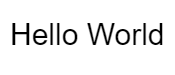
\includegraphics[width=\linewidth, frame]{figures/unzoomed-canvas.png}
        \caption{Canvas Image with Initial Size}
    \end{subfigure}
    \begin{subfigure}[b]{0.4\linewidth}
        \centering
        
\includegraphics[width=\linewidth, frame]{figures/zoomed-canvas.png}
        \caption{Canvas Image with Zoomed Size}
    \end{subfigure}
    \caption{Comparison of Unzoomed and Zoomed Canvas}
    \label{fig:canvas-zoom-comparison}
\end{figure}

In contrast with \code{canvas}, the \code{SVG} element does not have listed
problems. The term SVG (Scalable Vector Graphics) means an XML based vector
image format for defining 2D graphics. Therefore, as an element in HTML,
\code{SVG} simply represents a container for SVG graphics.

Because it is 'vector graphic', regardless of the ratio of rendered size and
programmed size, users can always get a clear graph of what they draw. This thus
solve the blurry problem of \code{canvas}.

\code{SVG} has several sub-element including \code{Path}. Data of a \code{Path} is a string containing commands and points, and is attached to its property 'd'. 

To show strokes that a user draws, instead of containing them in one \code{canvas} element, multiple \code{Path}s are used to display the user's drawing, each for one stroke. It is more flexible for the programme to monitor and control them. 

This feature fits \textit{React Component Lifecycle} perfectly as any change of path data causes React to 'react' to it, and render the path with updated data.

Overall, \code{SVG} is more suitable than \code{canvas} for this project due to its vector property and compatibility with React.

Before converting the Vanilla JS application to React component, an
existing React component, \textit{React-Sketch-Canvas}
\cite{react-sketch-canvas}, was investigated. It has most features this project
needs as a canvas, and can be directly installed in Lambda Feedback. However, it
only allows the user to erase on a stroke but cannot remove the whole stroke the
pointer points. The remove stroke function is considered important as the canvas
focuses more on writing than on drawing, and operations on strokes are more
important than on the graph. Besides, the existing component has many functions that are not needed but still need to be configured when invoking. Therefore, it was decided to develop a custom canvas with \code{SVG} so that necessary functions are included and the size of the component is minimised.



\section{Equation Recognition}
\label{bgEqnRecognition}
An equation recognition function is required for the project. The function needs
to correctly recognize the content which users draw as an equation. High accuracy is required for this project to ensure good user experience. In addition, response to recognition request should be quick so that live update is available.

Initially, building a model with machine learning was considered, and some tools
such as TensorFlow and Pytorch were preliminarily explored. It then turned out
that this approach is excessively time-consuming if a high-accuracy model is
wanted. Wenqi Zhao, etc.'s project \textit{Handwritten Mathematical Expression
Recognition with Bidirectionally Trained Transformer} \cite{zhao2021handwritten}
in 2021 shows that after 8 months of development and training, their model
achieved scores of 57.91\%, 54.49\%, and 56.88\% on three different datasets.
This apparently does not meet the high accuracy requirement. Although improvements can be made upon existing projects, it is still impossible to train a model with sufficient accuracy within 2 months, and this approach is discarded as a consequence.

As a result, the project finally uses an existing service for mathematical equation recognition: \textit{Mathpix}.

\begin{figure}[h]
    \centering
    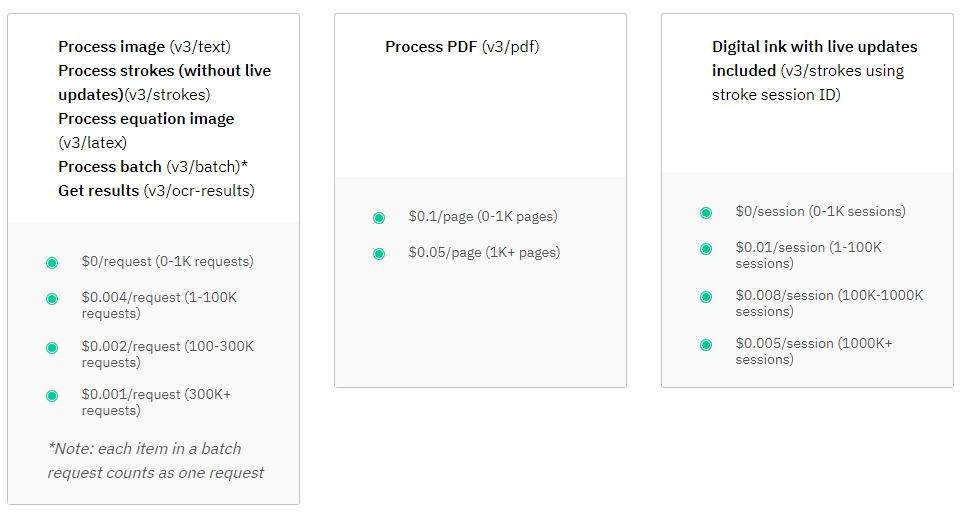
\includegraphics[width=\hsize]{figures/mathpix-pricing.png}
    \caption{Mathpix OCR API Pricing \cite{mathpix-pricing}}
    \label{fig:mathpix-pricing}
\end{figure}

\textit{Mathpix} is a company that focuses on mathematical equation recognition.
It provides OCR (Optical Charactor Recognition) APIs for developers so that they
can embed this feature in their project. Figure \ref{fig:mathpix-pricing} shows
the pricing of the service.

\textit{Mathpix} receives image data and recognizes the content in the image. If one or multiple equations are found, it can return the result in several styles like Latex, MathML and Asciimath etc. There are also options such as \code{confidence}, \code{data type} to assist the user for further process on the reponse data. In addition, it provides complete error messages which is helpful for development.

Although there are other companies providing similar services such as \textit{MyScript}, \textit{Mathpix} is advantageous at its \textit{App Token} and \textit{digital ink} method.

To request recognition, \textit{Mathpix} requires the \textit{API Key} to verify
if the access is authorised. Therefore, the \textit{API Key} must not be
included in the client end, or they can easily be stolen by hackers by
inspecting the app binary. This means that \textit{API Key} and corresponding
functions should be implemented in backend, and every time a recognition request
is made by client end, it is passed to the backend. The backend then makes the request to \textit{Mathpix} server and returns the response to the client end. This could waste time transmitting data, and bring much load to the backend server when multiple client ends make requests at the same time. 

To solve the problem, \textit{Mathpix} provides an \textit{App Token} function, which creates a short live client side token so that client apps can make request directly to \textit{Mathpix} server. In this approach, the clients no longer need to proxy their requests through the backend, but only need to request an \textit{App Token} from the backend. It largely reduces the time on data transmition and load of the backend server. 

Figure \ref{fig:comparison-key-token} illustrates the procedures of two methods mentioned above.
\begin{figure}[h]
    \centering
    \begin{subfigure}[c]{\hsize}
        \centering
        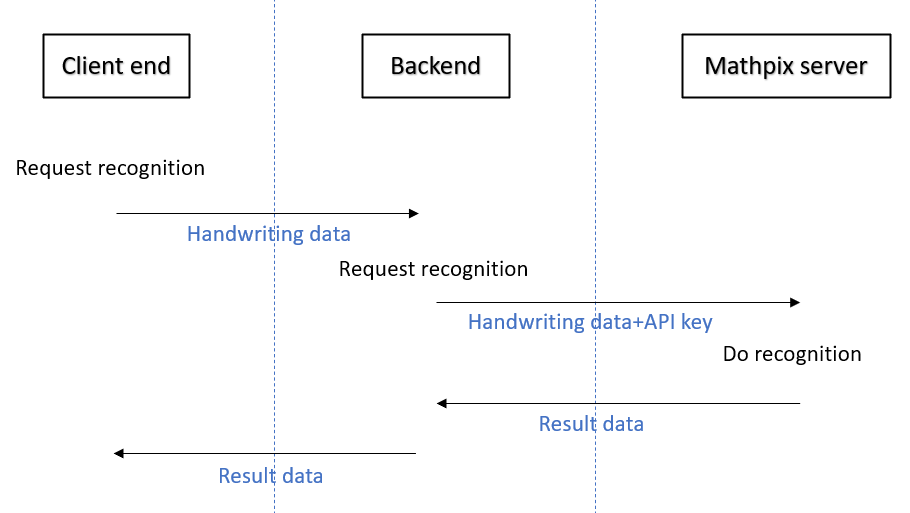
\includegraphics[width=\linewidth, frame]{figures/use-apikey.png}
        \caption{Use API Key for Recognition}
        \label{fig:use-apikey}
    \end{subfigure}
    \begin{subfigure}[c]{\hsize}
        \centering
        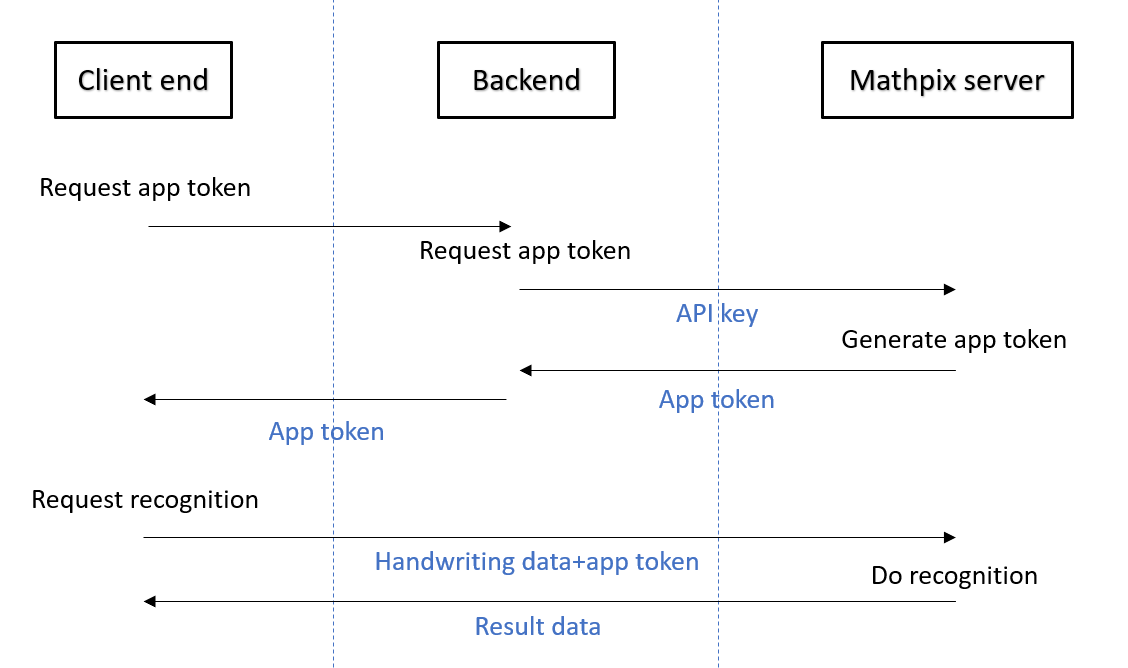
\includegraphics[width=\linewidth, frame]{figures/use-apptoken.png}
        \caption{Use App Token for Recognition}
        \label{fig:use-apptoken}
    \end{subfigure}
    \caption{Comparison of Using API Key and App Token for Recognition}
    \label{fig:comparison-key-token}
\end{figure}

While other services require the image to be uploaded in their API call,
\textit{Mathpix}'s \textit{digital ink} method allows users to upload stroke
data, i.e. coordinates of points on strokes, in their API call in order to
reduce network load and response time. Moreover, a live processing session for 5
minutes can be created in \textit{digital ink} method. In a session, users can
invoke APIs as many times as they but only counts once in pricing, which is much
more cost-effective.

In conclusion, \textit{Mathpix} is the best choice regarding accuracy, cost and time and development.

Another thing to be noted is the equation rendering. \textit{Mathpix} can return a latex styled string of the result, but the string cannot be displayed as an equation in web page. Therefore, a rendering tool is needed to parse the latex string and display the equation in the web page. 

This project uses \code{Katex}, which is the same tool used in \textit{Mathpix}. It can render a latex styled equation in one line of code \cite{web:katexapi}. Details will be 

This chapter records the background research on React framework, handwriting canvas to use and method of equation recognition, and givs reasons why \code{SVG} element and \textit{Mathpix} are used in the project. In Chapter \ref{Implementation}, the implementation of the Vanilla JS application, conversion to React component and integration with Lambda Feedback is explained.



%%%%%%%%%%%%%%%%%%%%%%%%%%%%%%%%%%%%
\chapter{Implementation}
\label{Implementation}

Following the three steps mentioned in Chapter \ref{Background}, this chapter is divided into three sections as well, each explaining the implementation of one step.

It should be noted that before installing the component into Lambda Feedback, the frontend part and backend part are not seperated for the convenience of development and test. This means that the Vanilla JS web application and React component contain the \textit{API Key} for requesting \textit{App Token}.

\section{Vanilla JS Web Application}
The first stage of the project is to develop a web application in Vanilla JS. This is to figure out the structure of the application and the working process of the programme, and focus on the JavaScript code but not React features.

The application
requests an \textit{App Token} when being launched. It has a handwriting area
for the user to draw, and when the user finishes a stroke, i.e. the pointer goes
up, it should automatically send the stroke data to \textit{Mathpix} server.
After receiving response from the serverm it should display the equation
recognised in text format. In addition, there should be a toolbar to edit the
content. 

This application consisits of three parts: 
\begin{itemize}
    \item Structure of the web pate (HTML)
    \item Functions (JavaScript)
    \item Styles of the web page (css file)
\end{itemize}

In this application, styles are not concerned as they will be specified in another approach in React. 

The structure of the web page is designed as Figure \ref{fig:vanillajs-structure}

\begin{figure}
    \centering
    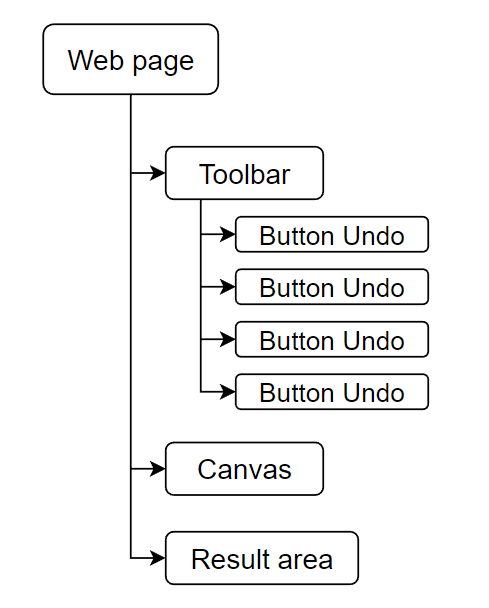
\includegraphics[width=0.5\linewidth, frame]{figures/vanillajs-structure.png}
    \caption{Structure of Vanilla JS Web Page}
    \label{fig:vanillajs-structure}
\end{figure}

The HTML code can thus be written easily based on the structure. It should be
noted that this application uses \code{canvas} element because \code{SVG}
element was not discovered yet when building this prototype. The next step is to
add functions to the application. 

Different from developing in other languages such as Python and C++, test
functions are normally not available for frontend development with
JavaScript/TypeScript. Tests are usually carried in the console of a browser. Therefore, the application was developed progressively. Functions were divided into several parts and each part was added after previous part passed tests:
\begin{enumerate}
    \item Users can draw on the canvas, and stroke data is recorded
    \item The application can send stroke data to \textit{Mathpix} and display the result
    \item Undo, redo, delete and remove functions are available
\end{enumerate}

Following sections will explain how each function was implemented.

\subsection{Drawing on the canvas}
Before start, the \code{canvas} should be initialised and referred. This is done in a \code{setupCanvas} function, which sets up variables such as size, stroke color and stroke width etc.

To let the users draw on the canvas and display the strokes they draw, function
\code{addEventListener} was used. This function can detect specified HTML event
(e.g. \code{onClick}, \code{onMouseDown} etc.) on an HTML element, and bind the
event to a custom function so that once the event happens on the element, the
corresponding function is called. The function is used in \code{setupCanvas} as well.

In \code{canvas} element, three events are being detected: 
\begin{itemize}
    \item \code{onMouseDown}: the mouse button is pressed down
    \item \code{onMouseMove}: the mouse is moving
    \item \code{onMouseUp}: the mouse is released
\end{itemize}

In this application, three events are connected to function
\code{handleMouseDown}, \code{handleMouseMove} and \code{handleMouseUp}
respectively. Operations in each function are shown in flowchart in Figure
\ref{fig:flowchart1}.

\begin{figure}[h]
    \centering
    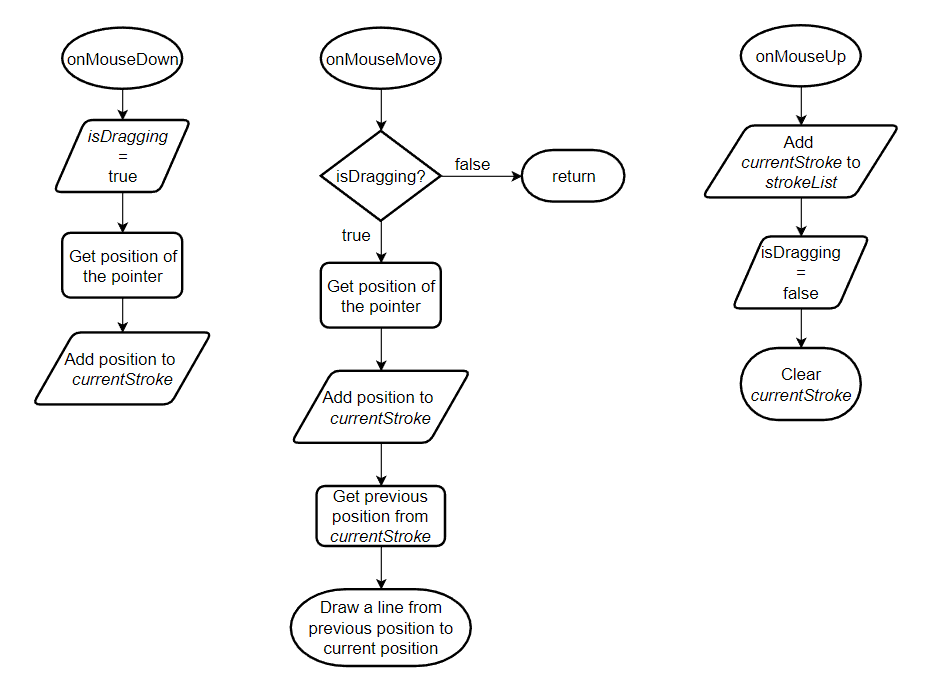
\includegraphics[width=\linewidth, frame]{figures/flowchart-op1.png}
    \caption{Event Flowcharts for Drawing on Canvas and Data Recording}
    \label{fig:flowchart1}
\end{figure}
Where:
\begin{itemize}
    \item \code{isDragging} is a state flag checking if the mouse is down
    \item \code{currentStroke} is a list of points representing the current stroke the user is drawing
    \item \code{strokeList} is a list of strokes representing all content the user has drawn, i.e. the stroke data
\end{itemize}

The function for \code{onMouseDown} sets a start point for the canvas to draw,
and marks the pointer state down. Event \code{onMouseMove} is checked every
browser's event loop. When it is detected, and mouse is down, the position of
the pointer is recorded to \code{currentStroke} and the \code{canvas} draws a
line from the previous point obtained from \code{currentStroke} and the current
position. This is done by methods \code{moveto(previousPoint)} and
\code{lineto(currentPoint)} of element \code{canvas}. 

The user can now draw paths on the canvas, and stroke data is recorded in this process. The next section will explain how stroke data is sent to \textit{Mathpix} and how result is fetched and displayed.

\subsection{Send stroke data and display result}
In this application, there are two requests to \textit{Mathpix}: \textit{App Token} request and recognition request. Both requests are made by \code{cURL}. In JS/TS, this can be done by \code{fetch} function. It can send a request through HTTP pipeline and fetch response asynchronously across the network \cite{web:fetchapi}. Using \code{fetch}, it is easy to make requests for \textit{App Token} and recognition.

\textit{App Token} should be obtained when the web page launches. Therefore, the
request is added in \code{setupCanvas} function. According to \textit{Mathpix}
document \cite{web:mathpixdoc}, the request header should include the \textit{API Key} for authorisation and content type of \code{application/json} for data transmission. The data to transmit is to ask the server to return session ID so that a live session is created. The \textit{Mathpix} server will then return an object containing \textit{APP Token} and \textit{session id}. The object is then parsed and data is stored.

As to recognition request, to realise live update, the content should be recognised every time the user finishes a stroke, which corresponds to the event \code{onMouseUp}. Therefore, the request is added to function \code{handleMouseUp}. 

Instead of \textit{API Key}, recognition request uses \textit{APP Token}. This
is for seperation of backend and frontend in further development. The data to
submit is the stroke data (\code{strokeList}) and \textit{session id}. Moreover,
options for the response can be specified in the data as well. In this
application, \code{latex\_styled} is included in the option so that a latex styled string is included in the result. \textit{Mathpix}
will process the data and return the result as an object containing required
data format. The object is then parsed and the \code{latex\_styled} result is stored.

After the result is obtained, it has to be displayed. As introduced in Chapter \ref{bgEqnRecognition}, \code{Katex} can render a latex styled string to equation in a specified element. In this application, it is rendered in the element \code{result area}. This is done after the result is obtained, which is in function \code{handleMouseUp} as well.

Now, the flowchart of function \code{handleMouseUp} becomes Figure \ref{fig:flowchart2}
\begin{figure}[h]
    \centering
    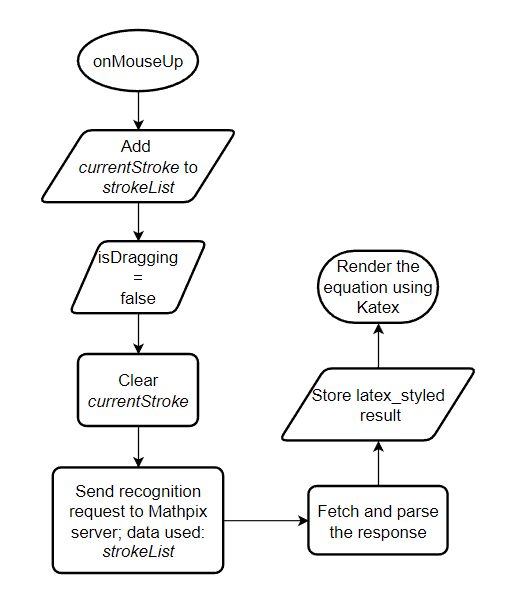
\includegraphics[width=0.6\linewidth]{figures/flowchart2.png}
    \caption{Flowchart of \code{handleMouseUp} for Recognition}
    \label{fig:flowchart2}
\end{figure}

This section records the implementation of recognition and render. The next section will explain how undo, redo, delete and remove functions are implemented.

\subsection{Toolbar functions}
Four edit functions, \code{undo}, \code{redo}, \code{delete} and \code{remove} are implemented in the toolbar. As \code{remove} function affects the development of \code{undo} and \code{redo} functions, it is implemented firstly.

The \code{remove} function is bound to the remove button. When the button is
clicked, the application enters the 'remove' mode: when the pointer presses on
or is dragged over a stroke, the stroke is removed. This is done by traversing
all points in all strokes, and compare them to the position where the pointer is
down. If horizontal and vertical difference is below a specific value, typically
\code{3*stroke width}, the stroke is moved from \code{strokeList} to \code{undoStrokeList},  the canvas
redraws all strokes and stroke data is submitted for recognition. This function
is named \code{checkCollision}, and the flowchart is shown in Figure \ref{fig:flowchart-remove}:
\begin{figure}[H]
    \centering
    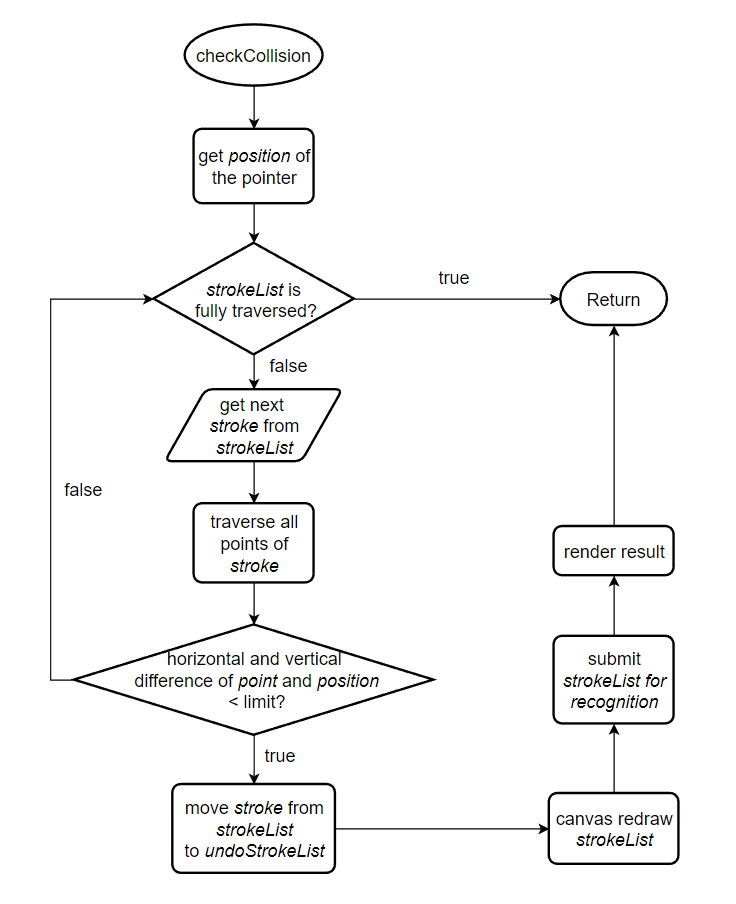
\includegraphics[width=0.8\linewidth, frame]{figures/flowchart-remove.png}
    \caption{Flowchart of Function \code{checkCollision}}
    \label{fig:flowchart-remove}
\end{figure}

It should be noted that when 'remove' mode is added to the application, a state flag \code{isDrawing} is added to check if it is in 'remove' mode. Every time \code{handleMouseDown} or \code{handleMouseMove} is invoked, \code{isDrawing} is checked to determine following operations. The flowchart of \code{handleMouseDown} and \code{handleMouseMove} thus becomes Figure \ref{fig:flowchart3}: 
\begin{figure}[H]
    \centering
    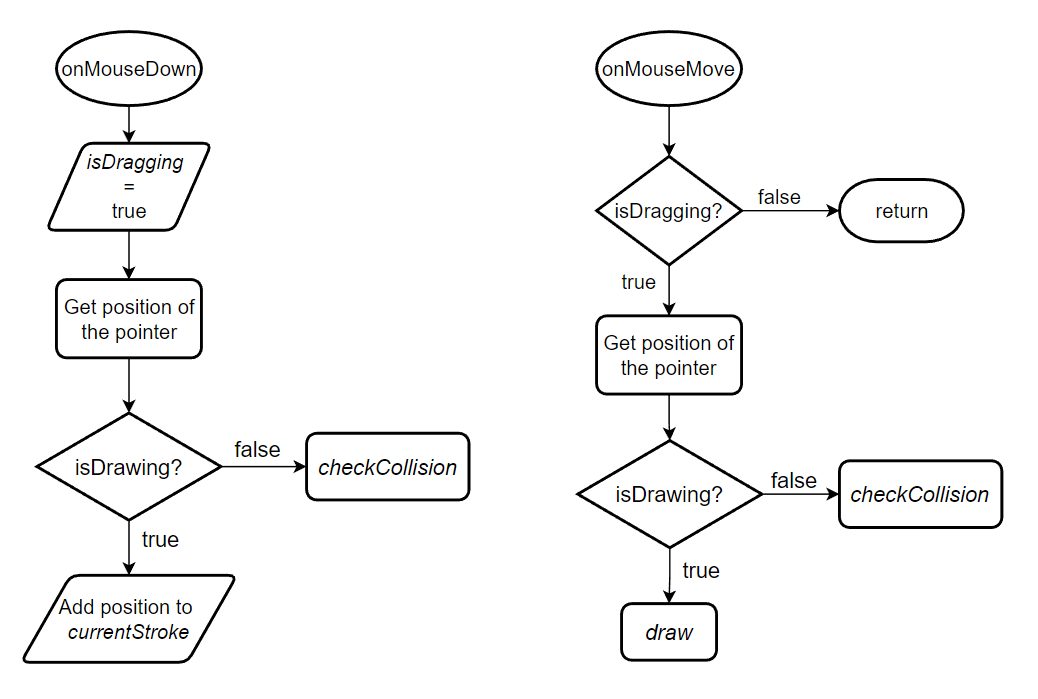
\includegraphics[width=\linewidth, frame]{figures/flowchart3.png}
    \caption{Flowchart of \code{handleMouseDown} and \code{handleMouseMove} with 'remove' mode}
    \label{fig:flowchart3}
\end{figure}
Where \code{draw} is illustrated in Figure \ref{fig:flowchart1}

Function \code{delete} simply clears the canvas and the stroke data, i.e. \code{strokeList}. Note that the result area is cleared as well.

Function \code{undo} depends on the operation done to determine whether to
remove or restore a stroke. Therefore, a variable named \code{operations} is
needed to record all operations. When a stroke is added to \code{strokeList},
string 'draw' is added to \code{operations}; when a stroke is removed from
\code{strokeList}, string 'remove' is added to \code{operations}. When
\code{undo} is invoked, it checks the last operation in \code{operations} and
moves it to \code{undoOperations}. If the last operation is 'add', the last
stroke in \code{strokeList} is moved to \code{undoStrokeList}; else, the last
stroke in \code{undoStrokeList} is moved to \code{strokeList}.

Two assist functions, \code{removeLastStroke} and \code{restoreLastStroke}, are
used. Flowcharts are shown in Figure \ref{fig:flowchart-helpfunc}.
\begin{figure}[h]
    \centering
    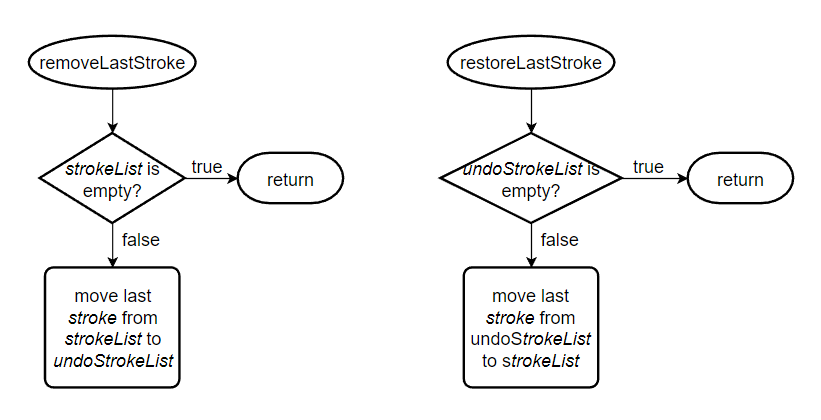
\includegraphics[width=\linewidth]{figures/flowchart-helpfunc.png}
    \caption{Flowchart of \code{removeLastStroke} and \code{restoreLastStroke}}
    \label{fig:flowchart-helpfunc}
\end{figure}

Function \code{redo} has opposite logic of \code{undo}, and can be easily implemented from it. Flowchart of \code{undo} and \code{redo} is shown in Figure \ref{fig:flowchart-undoredo}
\begin{figure}[H]
    \centering
    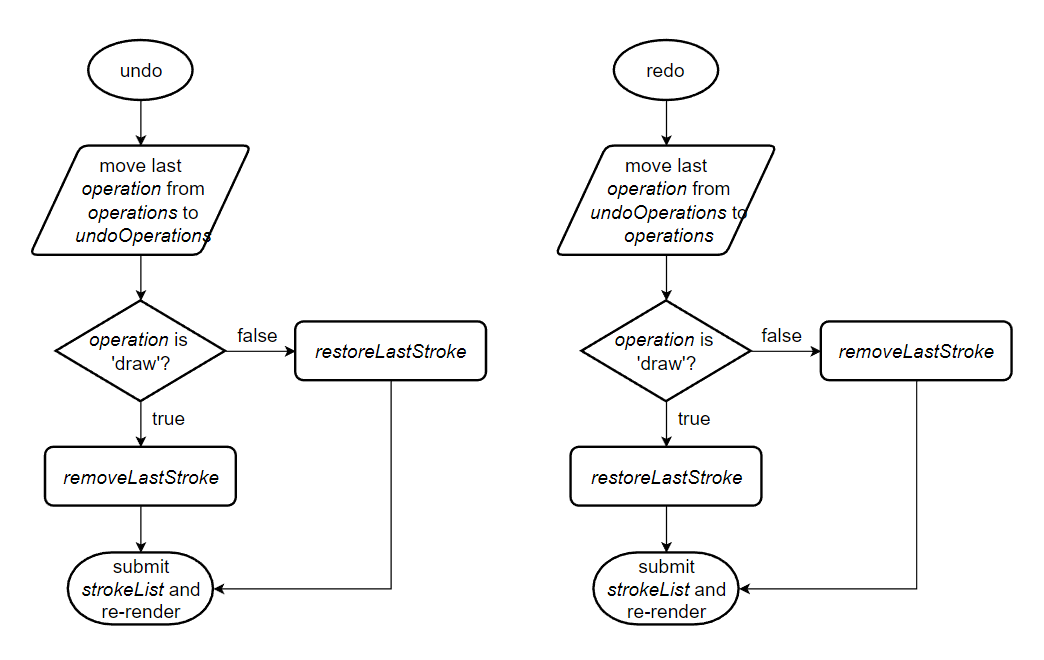
\includegraphics[width=\linewidth, frame]{figures/flowchart-undoredo.png}
    \caption{Flowchart of \code{undo} and \code{redo}}
    \label{fig:flowchart-undoredo}
\end{figure}

The implementation of the Vanilla JS web application is completed, and a test is carried out to validate that all functions are working. Figure \ref{fig:vanillajs-result} is a screenshot of the application.
\begin{figure}[h]
    \centering
    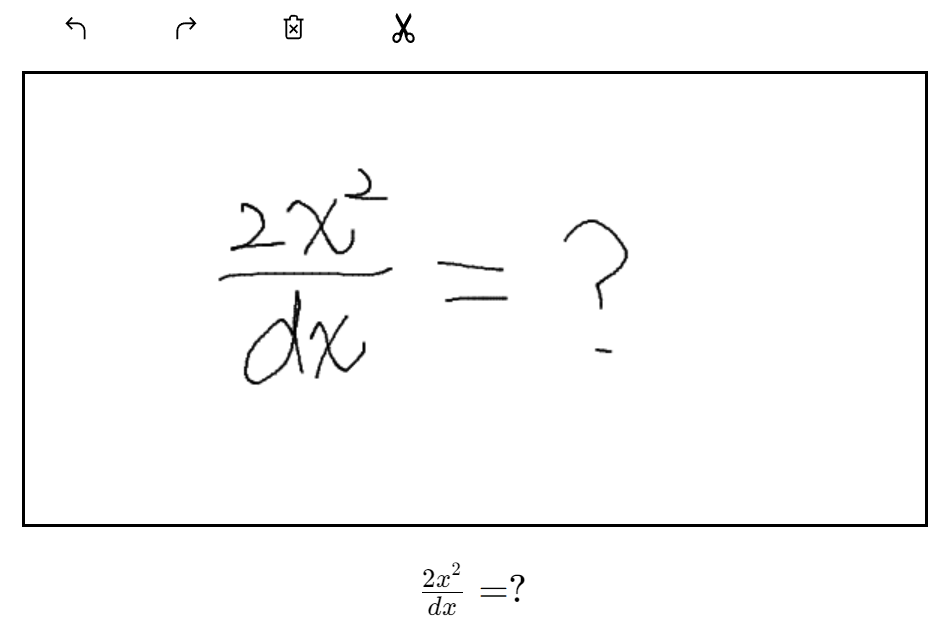
\includegraphics[width=\linewidth]{figures/vanillajs-result1.png}
    \caption{Screenshot of Vanilla JS Application}
    \label{fig:vanillajs-result}
\end{figure}

It can be seen from Figure \ref{fig:vanillajs-result} that though the application has realised all functions, the content in the writing area (\code{canvas}) is blurry. This will be fixed in the next step.

After examining the functionality of the application, the project moves to the next stage - conversion to React component. 

\section{Convert to React component}
\label{imp-react}
Now that the Vanilla JS application has implemented the required functions, this chapter will then discuss the conversion to React component to adapt to Lambda Feedback.

To convert from Vanilla JS to React component, the programme is restructured into sub-components according to functions:
\begin{itemize}
    \item \code{Canvas}: the area where users draw. 
    \item \code{FullScreenDialog}: a container to wrap the component so that it can be installed in Lambda Feedback.
    \item \code{Navbar}: the toolbar to place function buttons.
    \item \code{Path}: display one stroke
\end{itemize}

Besides, a type \code{Point} is created to represent the position of a point.

All sub-components are wrapped in a parent component \code{HandwritingInput},
where most functions are deployed. It receives events from sub-components, executing corresponding functions to the events and distribute the changes to sub-components. Variables in Vanilla JS application are included in the parent component as React state variables.
Figure \label{fig:react-component-structure} shows the structure of the component.

\begin{figure}[h]
    \centering
    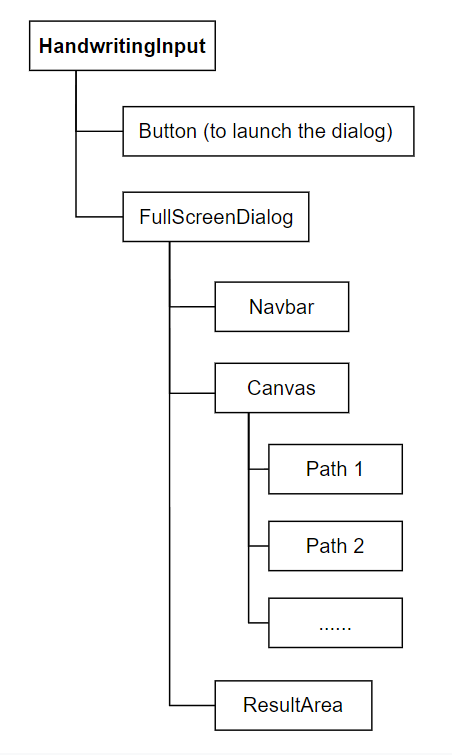
\includegraphics[width=0.6\linewidth]{figures/react-component-structure.png}
    \caption{Structure of the React Component}
    \label{fig:react-component-structure}
\end{figure}

It should be noted that for the handwriting area of the React component, the
\code{canvas} element is replaced with \code{SVG} element. This thus leads to a
new sub-component \code{Path}. This is the only change in the conversion in terms of implementation of functionalities. 

Similar to Vanilla JS, the React component is built in the order of functions.

\subsection*{Handwriting Area}
The logic of adding strokes to \code{strokeList} remains the same, but instead of using \code{addEventListner}, events and functions are bound via attributes. 

Component \code{HandwritingInput} has three functions, \code{handlePointerDown},
\code{handlePointerMove} and \code{handlePointerUp}, which have same
functionalities as handling functions in Vanilla JS app except for getting the position of the pointer, as this happens in \code{Canvas}. These functions are
passed to component \code{Canvas} as function typed attributes
\code{onPointerDown}, \code{onPointerMove} and \code{onPointerUp} respectively.
This allows \code{Canvas} to let \code{HandwritingInput} execute handling
functions by calling the 'on' functions inside \code{Canvas} component. 

In \code{Canvas}, three 'handle' functions are created, which gets the position of the pointer, and invoke the 'on' functions with the position as the parameter. Now, calling a 'handle' function inside \code{Canvas} does all functionalities same in Vanilla JS app.

To call 'handle' functions in response to a pointer event, they have to be bound
to the \code{SVG} element. The \code{SVG} element is created in the
\code{return} command. It also has \code{onPointerDown}, \code{onPointerMove}
and \code{onPointerUp} attributes, which can be bound to a function so that
everytime the 'on' attribute triggers (pointer down/move/up), the corresponding
function is called. 'Handle' functions in \code{Canvas} are then passed to attributes of the \code{SVG} element created inside. Thus, all functions that should react to an event are chained.
 
Figure \ref{fig:react-handwriting-area} shows the structure of the handwriting area.
\begin{figure}[h]
    \centering
    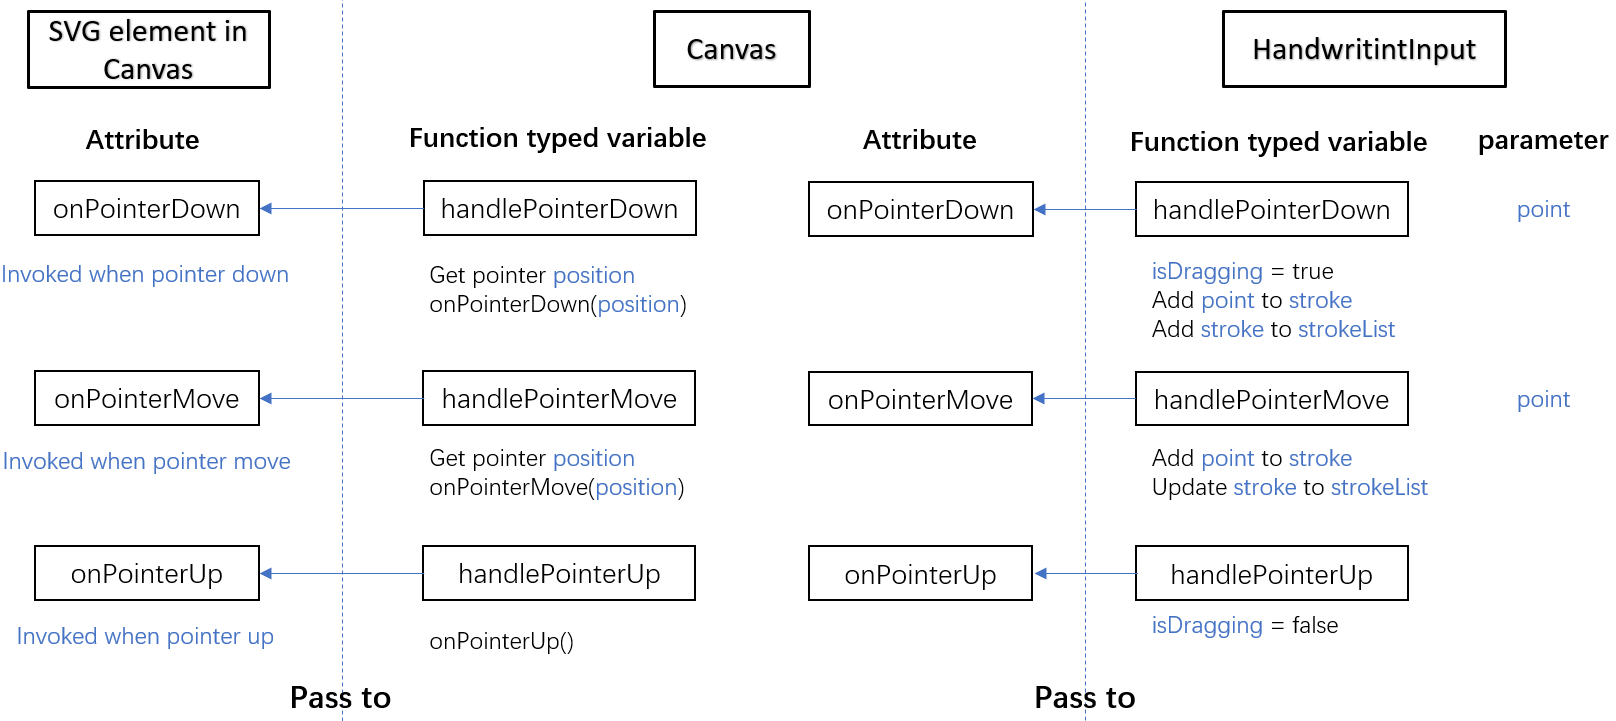
\includegraphics[width=\linewidth]{figures/react-handwriting-area.png}
    \caption{Structure of Handwriting Area in React Component}
    \label{fig:react-handwriting-area}
\end{figure}

It is worth noting that handlers in \code{HandwritingInput} does not draw
strokes like Vanilla JS app. This is because strokes in this component are
displayed by \code{Path} components inside \code{SVG} element, and when \code{strokeList} is updated, all
\code{Path}s update automatically. This is done by mapping \code{strokeList} to
\code{Path}s, each \code{Path} component is distributed a stroke from
\code{strokeList} with a key equal to the index of the stroke. Therefore, any
change made to \code{strokeList} will make React rerender the \code{Path}s.

\code{Path} component has an attribute named \code{stroke}, which receives an
array of type \code{Point}. Inside \code{Path}, \code{stroke} is parsed and a
string of path data is generated. Path data is then attached to the attribute of
element \code{path} so that the stroke is drawn.
\begin{figure}
    \centering
    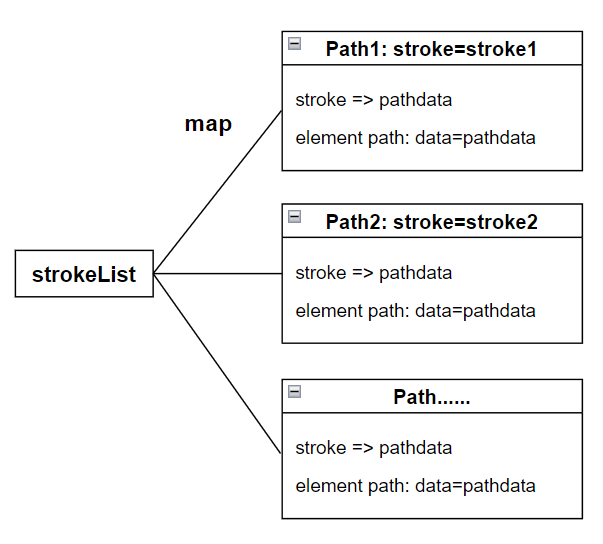
\includegraphics[width=0.8\linewidth]{figures/path-structure.png}
    \caption{Displaying Strokes}
    \label{fig:path-structure}
\end{figure}

Figure \ref{fig:path-structure} illustrates how \code{Path}s are generated and
strokes are displayed.

So far, the handwriting area has been converted to React component. The next step is to implement the equation recognition function.

\subsection*{Equation Recognition}
Same as Vanilla JS app, requests are made by \code{fetch} function. However,
stroke data is stored differently from Vanilla JS app in \code{strokeList}. In
previous stage, stroke data is stored in the method required by
\textit{Mathpix}, an example of one stroke \code{strokeList} is:

\centerline{\code{\{x: [x1, x2, x3...], y:[y1, y2, y3...]\}}}

However, to distribute strokes to \code{Path}, stroke data must be stroed like:

\centerline{\code{[Point1, Point2, Point3...]}}

Hence, a function \code{transformData} is written to transform \code{strokeList}
to \code{strokeUpload} with the data structure required by \textit{Mathpix}. This function is invoked in \code{undo}, \code{redo}, \code{remove} and \code{handleMouseUp}.

Another change made is that the request function is no longer called
\code{handleMouseUp} and three button functions. Instead, the React feature
\code{useEffect} on \code{strokeUpload}: when this variable changes, the request
function is called. A benifit of doing so is decreasing the couple between the
request function and the component, so that when the function needs to be
isolated, only a few code has to be maintained.

As to rendering the result, there is no difference with Vanilla JS app. The
component \code{ResultArea} receives a string of latex styled result as its
attribute, and uses Katex to render the string inside a \code{span} element. The
result string \code{renderString} is parsed from the response of recognition
request in \code{HandwritingInput} component.

Now that recognition part is finished, the toolbar and related functions are to be installed. 

\subsection*{Toolbar Implementation}
Methods \code{undo}, \code{redo}, \code{delete} and \code{remove} remain the same as Vanilla JS app. At this step, it is only necessary to consider how to transplant the methods to the component \code{Navbar}.

The \code{Navbar} has a MUI component \code{Appbar}, which aligns its sub-components in a toolbar. Here, four MUI component \code{Button}s are added, each representing one function.

Methods are implemented in \code{HandwritingInput} as they need data from the parent component. Therefore, to bind them with corresponding buttons, they are passed to the corresponding attribute, \code{onClick}, provided by each button. After that, each method can be called by clicking its button.

Functions are all implemented in the React component. However, it is still a web page as it is not wrapped. To work in Lambda Feedback, it must be wrapped so that it can be used as a component but not a web page.

\subsection*{Wrap the Component}
The component is wrapped in component \code{FullScreenDialog}. It contains a MUI component \code{Dialog}, and sets it to type 'fullScreen'. Using full screen is to provide enough space for the users to draw. A slide animation is added when opening the dialog so that it looks more fluent. 

The \code{FullScreenDialog} component wraps \code{Navbar}, \code{Canvas} and \code{ResultArea}, and is under \code{HandwritingInput}. A button is created to open the dialog.

The implementation of the React component is completed. A test was carried out
to check if the component works correctly. Figure
\ref{fig:react-component-webpage} shows that only a button displays when opening the React project - the component is wrapped.
\begin{figure}
    \centering
    
\includegraphics[width=0.4\linewidth, frame]{figures/react-component-button.png}
    \caption{React Component Web Page}
    \label{fig:react-component-webpage}
\end{figure}

%%%%%%%%%%%%%%%%%%%%%%%%%%%%%%%%%%%%
\chapter{Experimental Results}
\label{Results}


%%%%%%%%%%%%%%%%%%%%%%%%%%%%%%%%%%%%
\chapter{Conclusion}
\label{Conclusion}


%% bibliography
\bibliographystyle{vancouver}
\bibliography{mybibs}

\chapter{Appendices}
\label{Appendices}


\end{document}
